\documentclass[12pt]{beamer}
\usepackage{graphicx}
\usetheme{Warsaw} 

\author{Archana Kumari}
\title{MessAtt}
\subtitle{Mess Management System}
\date{May 2022}
\begin{document}

\begin{frame}
\maketitle
\end{frame}

\begin{frame}
    \frametitle{Agenda} 
             \begin{itemize}
             \item {Overview}
            % \item {Current Status}
             \item {Toolchain}
             \item {Short Demonstration}
             \item {Learnings}
             \item {Future Updates}
             \end{itemize}         
\end{frame} 

\begin{frame}
    \frametitle{What is MessAtt?}
    \begin{itemize}
        \item {MessAtt is a Facial Recognition Mess Management System, for serving food in hospital and hostel messes, ashrams and old homages.}
            \item{This system will ensure the one attendee can have at max one meal at a time.}
            \item{Also, it will help us keep a record of attendees who have received the meal.}
	\end{itemize}       
\end{frame}    
           
  
\begin{frame}
    \frametitle{Toolchains}
    \begin{itemize}          
        \item What are the Toolchains we used?
             \begin{itemize}
             \item { Python } 
      		 \item{face\_recognition library}
      		 \item { LaTeX } 
             
             \end{itemize}
             
       
    \end{itemize}       
\end{frame}  

\begin{frame}
    \frametitle{Short Demonstration}
    \begin{itemize}          
        \item {Let's have a look at a short demonstration of how MessAtt works.}                    
    \end{itemize}       
\end{frame} 

\begin{frame}  
  \frametitle{Capture image}      
      \begin {center}
         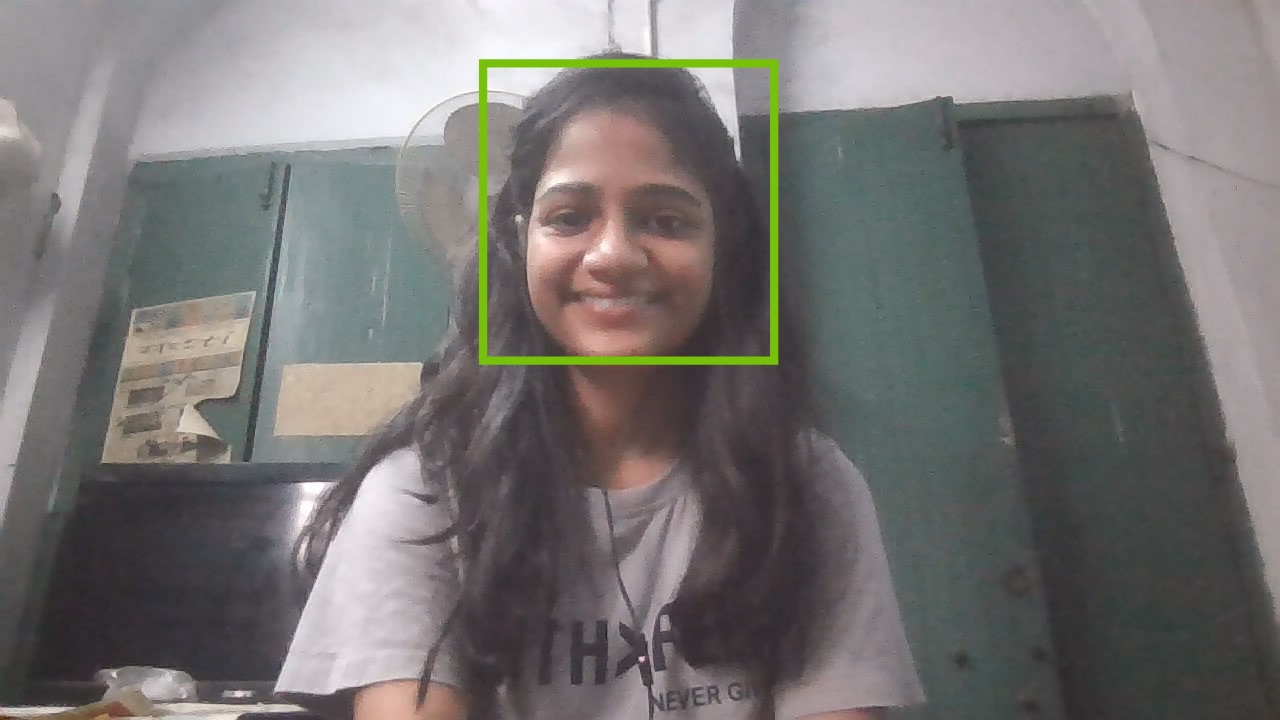
\includegraphics[scale=0.24]{archana.jpg} 
      \end{center}   
\end{frame}  

\begin{frame}  
  \frametitle{Stores Real Time Data in .csv file}      
      \begin {center}
         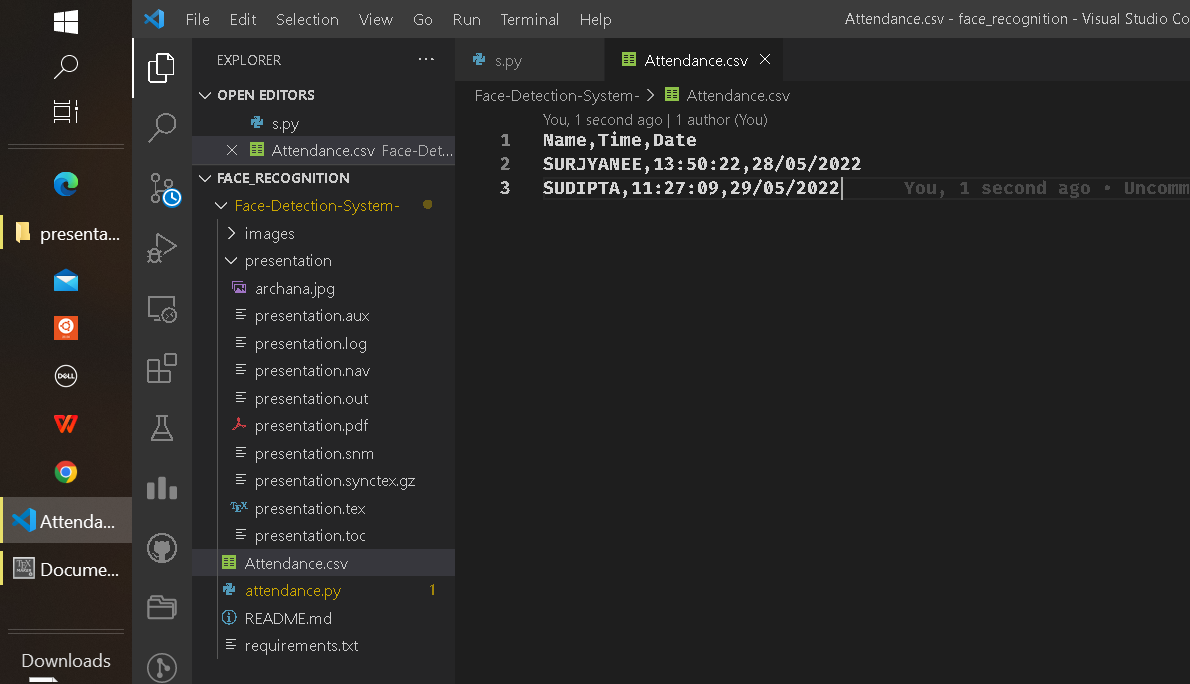
\includegraphics[scale=0.34]{storeData.png} 
      \end{center}   
\end{frame}   

\begin{frame}  
  \frametitle{Dataset of Images of Candidates}      
      \begin {center}
         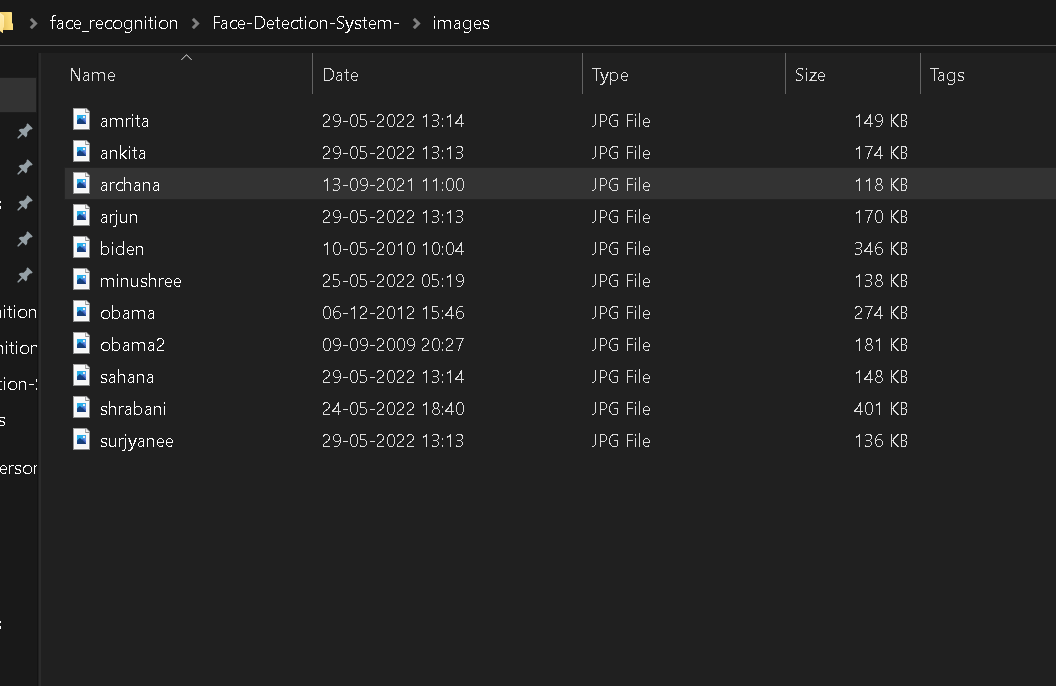
\includegraphics[scale=0.34]{data.png} 
      \end{center}   
\end{frame}   


\begin{frame}
    \frametitle{Learnings}
    \begin{itemize}          
        \item {Learnt how to implement facial recognition in real time.}
        \item{Explored new technologies in this regard.}
        \item{Learnt about Version Control System.}                    
        \item{Learnt about Time Management.}
    \end{itemize}       
\end{frame}

\begin{frame}
    \frametitle{Future Updates}
    \begin{itemize}          
        \item {Add a feature for ordering next day's meal in advance.}
        \item{Caculate monthly bills for each person. }                    
        \item{Add a feature for estimating the amount of the raw materials needed on each day (to avoid wastage).}
    \end{itemize}       
\end{frame}

\begin{frame}
    \frametitle{Thank You}
    \begin{itemize}           
        \item {Thank You}                    
    \end{itemize}     
      
\end{frame} 

\end{document}
